\section{Iterative Minimum Repairing}

\subsection{IMR}

\begin{frame}{\insertsubsection\ Intuition}
    \begin{block}{Intuitiver Ansatz von IMR}
        \begin{itemize}
            \item ARX nutzt markierte Werte effizient, \textbf{aber} ver�ndert die Werte zu drastisch.
            \item IMR Ansatz:
                \begin{enumerate}
                    \item Wende ARX an
                    \item W�hle \textbf{einen} Reparaturwert mit minimalen Abstand zur Messung
                    \item Wiederhole Prozedur bis aktuelle Reparatur sich nicht signifkant �ndert
                \end{enumerate}
            \item Motivation: Reparierte Werte verbessern zuk�nftige Reparaturen 
        \end{itemize}
    \end{block}
\end{frame}

\begin{frame}[fragile]{\insertsubsection\ = ARX + Minimum-Change-Prinzip}
    \begin{algorithm}[H]
    \begin{algorithmic}[1]
\STATE \textbf{Eingabe}: Messung $x$, markierte Werte $x^{\text{truth}}$, Ordnung $p$, Schwellenwert $\tau$ und max-num-iterations
\STATE \textbf{Ausgabe}: Reparatur $y$ 
        \STATE {$y^{(0)} \gets$ Initialize$(x,x^{\text{truth}})$}
\FOR{$k \gets 0$ \TO max-num-iterations}
\STATE {$\phi^{(k)} \gets$ Estimate$(x,y^{(k)})$}
    \STATE { $\hat{y} \gets$ Candidate$(x,y^{(k)}, \phi^{(k)})$}
    \STATE { $y^{(k+1)} \gets$ Evaluate$(x,y^{(k)}, \hat{y})$}
        \IF{ Converge($y^{(k)}, y^{(k+1)}$) }
        \STATE {\textbf{break}}
        \ENDIF
 \ENDFOR
    \RETURN $y^{(k)}$
\end{algorithmic}
\end{algorithm}
\end{frame}

\begin{frame}[fragile]{\insertsubsection:\ Initialisierung}
    \begin{algorithm}[H]
    \begin{algorithmic}[1]
\STATE \textbf{Eingabe}: Messung $x$, markierte Werte $x^{\text{truth}}$, Ordnung $p$, Schwellenwert $\tau$ und max-num-iterations
\STATE \textbf{Ausgabe}: Reparatur $y$ 
        \STATE \colorbox{blue!30}{{$y^{(0)} \gets$ Initialize$(x,x^{\text{truth}})$}}
\FOR{$k \gets 0$ \TO max-num-iterations}
\STATE {$\phi^{(k)} \gets$ Estimate$(x,y^{(k)})$}
    \STATE { $\hat{y} \gets$ Candidate$(x,y^{(k)}, \phi^{(k)})$}
    \STATE { $y^{(k+1)} \gets$ Evaluate$(x,y^{(k)}, \hat{y})$}
        \IF{ Converge($y^{(k)}, y^{(k+1)}$) }
        \STATE {\textbf{break}}
        \ENDIF
 \ENDFOR
    \RETURN $y^{(k)}$
\end{algorithmic}
\end{algorithm}
\end{frame}

\begin{frame}[fragile]{\insertsubsection:\ Initialisierung}
    \begin{block}{Initiale Reparatur}
        Initiale Reparatur $y^{(0)}$ ist Messung $x$ und �bernimmt die markierten Werte aus $x^{\text{truth}}$
    \end{block}
    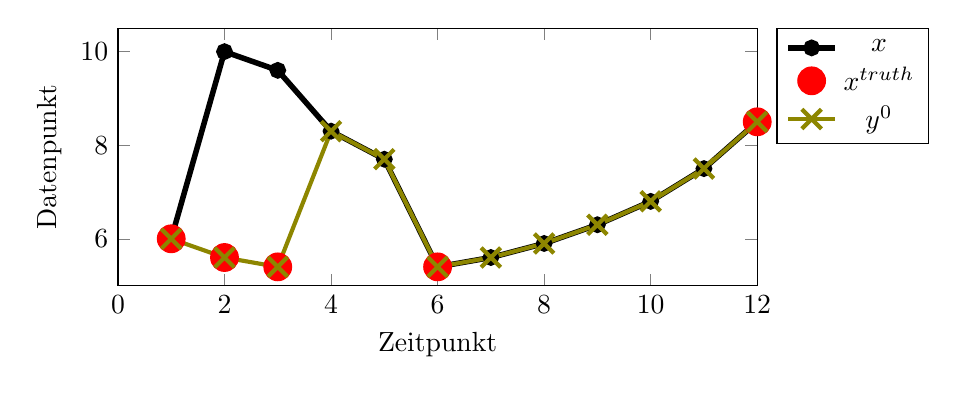
\begin{tikzpicture}
\begin{axis}[width=.8\textwidth,
   height=.4\textwidth,
xlabel=Zeitpunkt,
ylabel=Datenpunkt,
legend pos=outer north east,
xmin=0,
xmax=12,
ymin=5
]
\addplot[black, line width=2.0pt, mark size=2.0pt, mark=*]  table{
zeitpunkt wert 
1 6
2 10
3 9.6
4 8.3
5 7.7
6 5.4
7 5.6
8 5.9
9 6.3
10 6.8
11 7.5
12 8.5
};
\addlegendentry{$x$}
\addplot[only marks, red, mark size=5.0pt] table{
zeitpunkt wert 
1 6
2 5.6
3 5.4
6 5.4
12 8.5
};
\addlegendentry{$x^{\text{truth}}$}
    \addplot[olive,mark size=5.0pt, mark=x, line width=1.5pt] table{
    zeitpunkt wert 
    1 6
    2 5.6
    3 5.4
4 8.3
5 7.7
    6 5.4
    7 5.6
    8 5.9
    9 6.3
    10 6.8
    11 7.5
    12 8.5
    };
    \addlegendentry{$y^{0}$}
\end{axis}
\end{tikzpicture}

\end{frame}

\begin{frame}[fragile]{\insertsubsection: ARX auf aktuelle Reparatur anwenden}
    \begin{algorithm}[H]
    \begin{algorithmic}[1]
\STATE \textbf{Eingabe}: Messung $x$, markierte Werte $x^{\text{truth}}$, Ordnung $p$, Schwellenwert $\tau$ und max-num-iterations
\STATE \textbf{Ausgabe}: Reparatur $y$ 
        \STATE {$y^{(0)} \gets$ Initialize$(x,x^{\text{truth}})$}
\FOR{$k \gets 0$ \TO max-num-iterations}
        \STATE \colorbox{blue!30}{{$\phi^{(k)} \gets$ Estimate$(x,y^{(k)})$}}
        \STATE \colorbox{blue!30}{{ $\hat{y} \gets$ Candidate$(x,y^{(k)}, \phi^{(k)})$}}
    \STATE { $y^{(k+1)} \gets$ Evaluate$(x,y^{(k)}, \hat{y})$}
        \IF{ Converge($y^{(k)}, y^{(k+1)}$) }
        \STATE {\textbf{break}}
        \ENDIF
 \ENDFOR
    \RETURN $y^{(k)}$
\end{algorithmic}
\end{algorithm}
\end{frame}

\begin{frame}[fragile]{\insertsubsection:\ ARX auf aktuelle Reparatur anwenden}
    \begin{block}{Kandidaten}
        \begin{itemize}
            \item Parametersch�tzung $\phi$: aktuelle Reparatur $y^{(k)}$ wird als $x^{\text{truth}}$ interpretiert.
            \item Kandidaten $\hat{y}$ sind neue Reparaturwerte
        \end{itemize}
    \end{block}
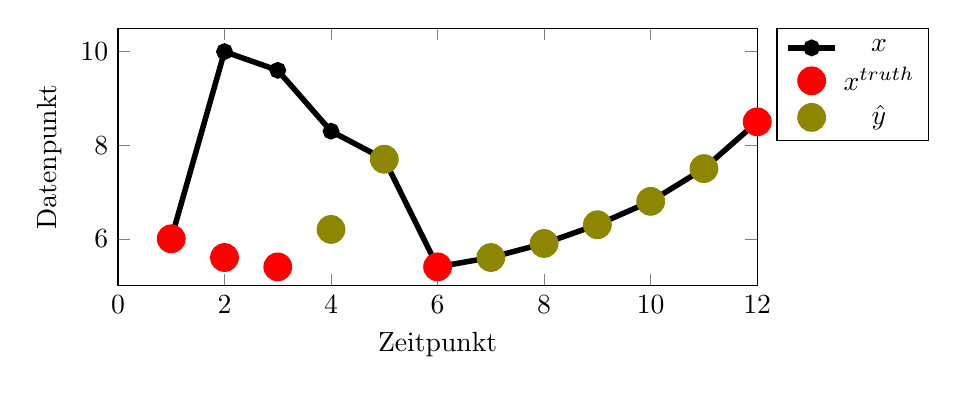
\begin{tikzpicture}
\begin{axis}[width=.8\textwidth,
   height=.40\textwidth,
xlabel=Zeitpunkt,
ylabel=Datenpunkt,
legend pos=outer north east,
xmin=0,
xmax=12,
ymin=5
]
\addplot[black, line width=2.0pt, mark size=2.0pt, mark=*]  table{
Zeitpunkt Wert 
1 6
2 10
3 9.6
4 8.3
5 7.7
6 5.4
7 5.6
8 5.9
9 6.3
10 6.8
11 7.5
12 8.5
};
\addlegendentry{$x$}
\addplot[only marks, red, mark size=5.0pt] table{
Zeitpunkt Wert 
1 6
2 5.6
3 5.4
6 5.4
12 8.5
};
\addlegendentry{$x^{\text{truth}}$}
\addplot[only marks, olive,mark size=5.0pt] table{
Zeitpunkt Wert 
4 6.2
5 7.7
7 5.6
8 5.9
9 6.3
10 6.8
11 7.5
};
   \addlegendentry{$\hat{y}$}
% if you have the file, you can do
% \addplot table {datafile.csv};
\end{axis}
\end{tikzpicture}

\end{frame}

\begin{frame}[fragile]{\insertsubsection: Minimum-Change}
    \begin{algorithm}[H]
    \begin{algorithmic}[1]
\STATE \textbf{Eingabe}: Messung $x$, markierte Werte $x^{\text{truth}}$, Ordnung $p$, Schwellenwert $\tau$ und max-num-iterations
\STATE \textbf{Ausgabe}: Reparatur $y$ 
        \STATE {$y^{(0)} \gets$ Initialize$(x,x^{\text{truth}})$}
\FOR{$k \gets 0$ \TO max-num-iterations}
\STATE {$\phi^{(k)} \gets$ Estimate$(x,y^{(k)})$}
    \STATE { $\hat{y} \gets$ Candidate$(x,y^{(k)}, \phi^{(k)})$}
        \STATE { \colorbox{blue!30}{$y^{(k+1)} \gets$ Evaluate$(x,y^{(k)}, \hat{y})$}}
        \IF{ Converge($y^{(k)}, y^{(k+1)}$) }
        \STATE {\textbf{break}}
        \ENDIF
 \ENDFOR
    \RETURN $y^{(k)}$
\end{algorithmic}
\end{algorithm}
\end{frame}

\begin{frame}[fragile]{\insertsubsection:\ Minimum-Change}
    \begin{block}{Minimum-Change}
        \begin{itemize}
            \item Zu geringe �nderungen werden herausgefiltert $|y^{(k)}_i - \hat{y}_i| > \tau$
            \item Geringste �nderung zu Messung $x$ wird als Kandidat ausgew�hlt
        \end{itemize}
    \end{block}
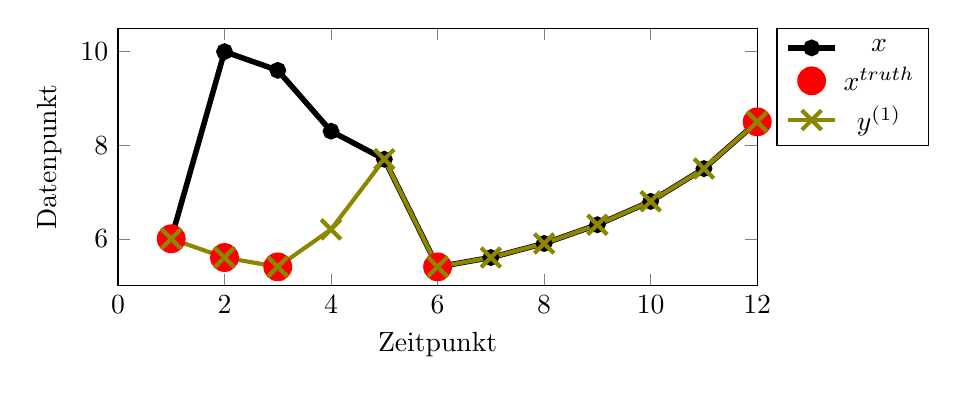
\begin{tikzpicture}
\begin{axis}[width=.8\textwidth,
   height=.40\textwidth,
xlabel=Zeitpunkt,
ylabel=Datenpunkt,
legend pos=outer north east,
xmin=0,
xmax=12,
ymin=5
]
\addplot[black, line width=2.0pt, mark size=2.0pt, mark=*]  table{
Zeitpunkt Wert 
1 6
2 10
3 9.6
4 8.3
5 7.7
6 5.4
7 5.6
8 5.9
9 6.3
10 6.8
11 7.5
12 8.5
};
\addlegendentry{$x$}
\addplot[only marks, red, mark size=5.0pt] table{
Zeitpunkt Wert 
1 6
2 5.6
3 5.4
6 5.4
12 8.5
};
\addlegendentry{$x^{\text{truth}}$}
\addplot[olive,mark size=5.0pt, mark=x, line width=1.5pt] table{
Zeitpunkt Wert 
    1 6
    2 5.6
    3 5.4
4 6.2
5 7.7
    6 5.4
7 5.6
8 5.9
9 6.3
10 6.8
11 7.5
12 8.5
};
    \addlegendentry{$y^{(1)}$}
% if you have the file, you can do
% \addplot table {datafile.csv};
\end{axis}
\end{tikzpicture}

\end{frame}

\begin{frame}[fragile]{\insertsubsection: Terminierung}
    \begin{algorithm}[H]
    \begin{algorithmic}[1]
\STATE \textbf{Eingabe}: Messung $x$, markierte Werte $x^{\text{truth}}$, Ordnung $p$, Schwellenwert $\tau$ und max-num-iterations
\STATE \textbf{Ausgabe}: Reparatur $y$ 
        \STATE {$y^{(0)} \gets$ Initialize$(x,x^{\text{truth}})$}
        \FOR{\colorbox{blue!30}{$k \gets 0$ \TO max-num-iterations}}
\STATE {$\phi^{(k)} \gets$ Estimate$(x,y^{(k)})$}
    \STATE { $\hat{y} \gets$ Candidate$(x,y^{(k)}, \phi^{(k)})$}
    \STATE { $y^{(k+1)} \gets$ Evaluate$(x,y^{(k)}, \hat{y})$}
        \IF{\colorbox{blue!30}{Converge($y^{(k)}, y^{(k+1)}$) }}
        \STATE {\colorbox{blue!30}{\textbf{break}}}
        \ENDIF
 \ENDFOR
    \RETURN $y^{(k)}$
\end{algorithmic}
\end{algorithm}
\end{frame}

\begin{frame}{\insertsubsection: Terminierung}
    \begin{block}{Terminierung}
        \begin{itemize}
            \item Zwei M�glichkeiten der Terminierung:
        \begin{itemize}
            \item Maximale Anzahl der Iterationen wird erreicht
            \item Konvergenz: Neue Reparatur $y^{(k+1)}$ ist gleich aktuelle Reparatur $y^{(k)}$
        \end{itemize}
    \item Allgemeine Konvergenzfrage ist noch offen
        \end{itemize}
    \end{block}

\end{frame}

\subsection{Optimierung 1: Matrix-Pruning IMR}
\begin{frame}{Motivation von Matrix-Pruning IMR}
    \begin{block}{Laufzeit- \& Platzproblem}
        \begin{itemize}
            \item Parametersch�tzung beansprucht viel Zeit und Platz
            \item Matrizen V und Z bestehen aus $y_i^{(k)} - x_i$:
                \begin{itemize}
                    \item wenige markierte Werte vorhanden
                    \item markierte Werte h�ufig identisch zur Messung
                    \item Reparaturwerte �ndern sich nicht signifkant
                    \item $\rightarrow$ d�nnbesetzte Matrizen
                \end{itemize}
            \item Matrix-Pruning: L�schen von Zeilen mit 0en
        \end{itemize}
    \end{block}
\end{frame}

\begin{frame}{Matrix Pruning IMR Beispiel}
    \begin{block}{Beispiel}
        Zeilen mit 0en in Z und entsprechende Zeile in V sind entfernbar:
        \[
            Z =
            \left(
\begin{array}{c}
0\\
-4.4\\
-4.2\\
0\\
0\\
0\\
0\\
0\\
0\\
0\\
0\\
\end{array}
\right)
            V =
            \left(
\begin{array}{c}
-4.4\\
-4.2\\
0\\
0\\
0\\
0\\
0\\
0\\
0\\
0\\
0\\
\end{array}
\right)
\rightarrow
            Z_{mp} =
            \left(
\begin{array}{c}
-4.4\\
-4.2\\
\end{array}
\right)
            V_{mp} =
            \left(
\begin{array}{c}
-4.2\\
0\\
\end{array}
        \right)
        \]
    \end{block}
\end{frame}
\subsection{Optimierung 2: Inkrementelle Berechnung}
\begin{frame}{Inkrementelle Berechnung (IMR-IC)}
\begin{block}<-+>{Intuition}
\begin{itemize}
\item IMR Algorithmus berechnet $\phi^k$ in jede Iteration $k$
\[\phi^k \leftarrow  Estimate(x , y^k)\]
\item Minimum-Change-Prinzip, ein Wert $r$ wird ge�ndert 
\[y^k_r\neq y^{k-1}_r\]
\item Fast alle Werte in $Z^k,Z^{k-1}$ und $V^k, V^{k-1}$ bleiben unver�ndert
\end{itemize}
\end{block}
\end{frame}
\begin{frame}{Inkrementelle Berechnung (IMR-IC)}
\begin{block}{Rekursive Formel}
Sei $\phi^{(k)} = (A^{(k)})^{-1}B^{(k)}$ mit $A^{(k)}=(Z^{(k)})'Z^{(k)}$ und $B^{(k)}=(Z^{(k)})'V^{(k)}$
\end{block}
\begin{block}{Fall: $1\leq i \leq p$}
\[a_{ii}^{(k)}=a_{ii}^{(k-1)} + \begin{cases}
0 &falls\, r<p+1-i\vee r>n-i\\
z_r^{(k)}z_r^{(k)}-z_r^{(k-1)}z_r^{(k-1)} &falls\, p+1-i\leq r\leq n-i
\end{cases}
\]
\end{block}
\end{frame}

\begin{frame}{Inkrementelle Berechnung (IMR-IC)}
\begin{block}{Fall: $1\leq i \leq p$, $1\leq j \leq p$, $i<j$}
\[a_{ij}^{(k)}=a_{ji}^{(k)}=a_{ij}^{(k-1)}+ (z_r^{(k)}-z_r^{(k-1)}) \times\]
\[
\begin{cases}
0 &falls\, r<p+1-j\vee r>n-i\\
z_{r+j-i}^{(k-1)}&falls\, p+1-j\leq r < p+1-i\\
z_{r-j+i}^{(k-1)}&falls\, n-j<r\leq n-i\\
(z_{r+j-i}^{(k-1)} + z_{r-j+i}^{(k-1)})&falls\, p+1-i\leq r\leq n-i
\end{cases}
\]
\end{block}
\end{frame}

\begin{frame}{Inkrementelle Berechnung (IMR-IC)}
\begin{block}{Fall: $1\leq i \leq p$}
\[b_{i}^{(k)}=b_{i}^{(k-1)}+ (z_r^{(k)}-z_r^{(k-1)}) \times\]
\[
\begin{cases}
0 &falls\, r<p+1-i\vee r>n-i\\
z_{r+i}^{(k-1)}&falls\, p+1-i\leq r < p+1\\
z_{r-i}^{(k-1)}&falls\, r> n-i\\
(z_{r+i}^{(k-1)} + z_{r-i}^{(k-1)})&falls\, p+1\leq r\leq n-i
\end{cases}
\]
\end{block}
\end{frame}

\begin{frame}[fragile]{Rekursive Algorithmus}
    \begin{algorithm}[H]
    \begin{algorithmic}[1]
\STATE \textbf{Eingabe}: Messung $x$, Reparatur/Label $y$
\STATE \textbf{Ausgabe}: $\phi^{(k)}$
        \IF{$k=0$}
            \STATE Init $A^{(0)}$,$B^{(0)}$ mit $Z^{(0)}$, $V^{(0)}$
        \ELSE
            \STATE $r$ Index $y_r^{(k)}\neq y_r^{(k-1)}$ 
            \STATE Erstelle $A^{(k)}$, $B^{(k)}$ mit hilfe von $A^{(k-1)}$ und $B^{(k-1)}$ nach rekursive Formeln
        \ENDIF
        \STATE $\phi^{(k)}$ $\gets$ $(A^{(k)})^{-1}B^{(k)}$ 
\RETURN $\phi^{(k)}$
\end{algorithmic}
\end{algorithm}
\end{frame}



